% web10 paper — SECOND DRAFT: a fresh approach from the top.
% Same verified evidence as the first draft, re-derived from the thesis spine:
% a fresh structure (data plane split out, "Lessons from Running It" added),
% the same title, figures, table data, and artifact pins.
% Render: tectonic main.tex  (from this directory)
\documentclass[sigconf, nonacm]{acmart}
\settopmatter{printfolios=true} % Native ACM bottom-center numbers, including page one.
% Lower folios by half an inch without changing the text block or page breaks.
\AtBeginDocument{\addtolength{\footskip}{36pt}}

% --- packages (all in the tectonic bundle) ---
\usepackage{booktabs}
\usepackage{enumitem}
\usepackage{microtype}
% Give narrow columns a fallback line-breaking pass without changing margins.
\setlength{\emergencystretch}{2em}
\usepackage{xcolor}
\usepackage{listings}
\usepackage{graphicx}
\usepackage{tikz}
\usetikzlibrary{positioning,calc,arrows.meta}

% Brand tokens (knowledge-base/strategy/design.md §13)
\definecolor{web10bg}{HTML}{09090b}
\definecolor{web10fg}{HTML}{fafafa}
\definecolor{web10brand}{HTML}{8b5cf6}
\definecolor{web10brand300}{HTML}{c4b5fd}
\definecolor{web10muted}{HTML}{27272a}

% Pin implementation links and source-size accounting to the reviewed snapshot.
\newcommand{\artifactbase}{https://github.com/jacoby149/web10}
\newcommand{\artifactrev}{317fa349eae714ddde07f249ca65cdaa34b6459b}
\newcommand{\artifactdir}[2]{\href{\artifactbase/tree/\artifactrev/#1}{#2}}
\newcommand{\artifactfile}[2]{\href{\artifactbase/blob/\artifactrev/#1}{#2}}
% Domain prototype: immutable tested code/receipt publication, separate from size snapshot.
\newcommand{\domainartifactrev}{26720acba859c7eb03fc5d26a6221cdde5b764a1}
\newcommand{\domainartifactdir}[2]{\href{\artifactbase/tree/\domainartifactrev/#1}{#2}}

\lstdefinestyle{sql}{
  language={},
  basicstyle=\ttfamily\footnotesize,
  breaklines=true,
  frame=single,
  framesep=4pt,
  rulecolor=\color{gray!50},
  backgroundcolor=\color{gray!6},
  keywordstyle=\bfseries,
}
\lstdefinestyle{json}{
  language={},
  basicstyle=\ttfamily\footnotesize,
  breaklines=true,
  frame=single,
  framesep=4pt,
  rulecolor=\color{gray!50},
  backgroundcolor=\color{gray!6},
}

% --- acmart metadata ---
\setcopyright{none}
\acmConference[SIGMOD 2027 Industry Track]{SIGMOD 2027 Industry Track}{}{}
\acmPrice{}
\acmISBN{}
\acmDOI{}

\title{Your Data, Your Rules: \\ Extending the Decentralized Web}
\author{Jacob Hoffman}
\affiliation{\institution{web10 Inc.}\country{}}
\email{jacob@web10.app}

\begin{document}

\begin{abstract}
Email decentralized where your data \emph{goes}: a global identifier,
sovereign provider stores, and standardized transport---no central authority,
no shared mailbox. It never decentralized who may \emph{access} it: the
payload crossed provider boundaries, but the permissions did not. We present
\textbf{web10}, a deployed, user-addressed data platform that extends the
email model in both directions at once. Any application defines its own
document services over a shared columnar store, and a uniform, user-managed
access model lets a principal on any node hold a role in a user's groups.
The node enforces access at the query boundary: application-written SQL
resolves service names to reader-filtered relations \emph{before} joins and
aggregation execute. Clients read other nodes' data directly against each
node's verified-token API rather than through server-to-server content
federation. We report connected evidence: a game and a marketplace that reuse
the social application's profiles without a node change; an isolated
two-node experiment exercising foreign-principal grants and local revocation
under cached home-node certification; a browser prototype that keeps a public
domain subscription alive after the original provider goes dark; and a
metadata fan-out measurement that exposes the access layer's cost structure
and drives its batching decision.
\end{abstract}

\maketitle
%=============================================================================
\section{Introduction}
\label{sec:intro}

Email is the decentralized web's proof of concept. A global identifier
(\texttt{you@provider}), a sovereign store per provider, and standardized
server-to-server transport let a message cross providers with no central
authority and no shared mailbox database. The protocol and the identifier are
what make the network work; each provider's server is independent.

But email decentralized the \emph{data plane} for exactly one format---and it
never decentralized \emph{access}. You can email a Yahoo user from Gmail, but
you cannot grant that Yahoo user \emph{editor} on your Google Calendar. The
payload crossed the boundary; the permissions did not. Every social platform
inherits the same split at larger scale: the content is portable in principle,
while who follows whom, who belongs to which group, and who may read or
contribute stay locked inside the platform's backend.

\textbf{web10} extends the email model in two directions at once. First, the
data plane generalizes from one format to \emph{all} formats: a shared
columnar store in which any application defines its own services and its own
queries, so a post, a profile, a game score, and a marketplace listing are all
documents in the same store, addressed by the same primitives. Second, and
more consequentially, the \emph{access layer} is decentralized: a uniform,
user-managed permission vocabulary in which a grant is a row naming a
\emph{globally addressable principal} (\texttt{provider/username}), a group,
a service, and an operation. Any principal on any node can hold any role in a
group. The user is the policy administrator for their own data---and that
policy reaches across the network. Email let your data leave the building;
web10 lets your \emph{permissions} leave it too.

\begin{table}[t]
\caption{Capability comparison. Email is the model web10 generalizes, not a
social system. The entries summarize the models discussed in the cited work,
not an exhaustive survey of implementations. web10's column describes its
architecture; production cross-node integration remains incomplete.}
\label{tab:capabilities}
\centering
\scriptsize
\setlength{\tabcolsep}{5pt}
\begin{tabular}{@{}p{3.6cm}ccccc@{}}
\toprule
\textbf{Capability} & \textbf{Email} & \textbf{Masto-} & \textbf{Blue-} & \textbf{Solid} & \textbf{web10} \\
 & & \textbf{don} & \textbf{sky} & & \\
\midrule
User-owned data, portable & $\sim$ mail & $\sim$ & $\checkmark$ & $\checkmark$ & $\checkmark$ any \\
Fine-grained, user-mgmt access & $\times$ & $\times$ & $\times$ & $\sim$ res. & $\checkmark$ role \\
Access cross-node-addr. & $\sim$ addr & $\times$ & $\times$ & $\sim$ Pod & $\checkmark$ \\
Composable, app-def.\ query & $\times$ & $\times$ & $\sim$ view & $\sim$ dep. & $\checkmark$ SQL \\
User-addr.\ net.\ (no fed.) & $\checkmark$ & $\times$ & $\times$ & $\checkmark$ & $\checkmark$ \\
\bottomrule
\end{tabular}
\end{table}

Table~\ref{tab:capabilities} compares the systems discussed in this paper---
and the email model web10 generalizes---across five capabilities. The marks
are \checkmark\ (present), $\times$ (absent), or $\sim$ (partial / scoped).
The pattern is the email split, repeated. Mastodon~\cite{activitypub2018} and
Bluesky~\cite{kleppmann2024} let you follow someone on another server and
carry your data in principle, but their authorization is platform-defined and
coarse-grained---follow/block and collection-level visibility, not
per-principal grants over application-defined services. Facebook scales the
data plane to a massive lakehouse but keeps the access model entirely inside
its own platform. Solid~\cite{solid2016} is the closest prior work: it
decentralizes data \emph{and} some access, with WAC group
agents~\cite{wac2022} and ACP client/issuer matchers~\cite{acp2022}---but
its access model is \emph{resource-centric} (ACLs on linked-data resources)
rather than a uniform role/grant vocabulary over services that applications
define, and its cross-Pod query cost depends on deployment. web10 combines a
service-scoped permission model with application-defined SQL and
client-mediated cross-node reads. The comparison concerns these design
choices, not an exhaustive claim of functional exclusivity or a measured
advantage over the other systems.

The platform is deployed and serving real users. web10-social is a
creator-oriented social application---feeds, groups, direct messages,
discovery, short- and long-form video, music---and its persistent data and
authentication live entirely in the generic node: no separate social-data
backend. The node also serves two small static applications, a game and a
marketplace, that read the social application's \texttt{profile} documents
through the same access boundary. No node change, no application-specific
endpoint, no API agreement between the applications. That last sentence is
the point of this paper.

This paper makes three contributions:

\begin{enumerate}[leftmargin=*,nosep]
  \item \textbf{A user-addressed network model} (\S\ref{sec:network}): a
  federation of sovereign nodes in which the user's client mediates
  cross-node reads, each node re-authorizes every read against a verified
  token, and the access model is globally addressable by construction---
  generalizing email from one data format to all formats and from content
  routing to access control.
  \item \textbf{A reader-specific query boundary} (\S\ref{sec:enforcement}):
  application-written SQL over a shared columnar store, in which service
  references resolve to reader-filtered CTEs \emph{before} the caller's joins
  and aggregation---the access decision is made on the input, not patched
  onto the output.
  \item \textbf{A deployed platform with a measured cost structure}
  (\S\ref{sec:platform}--\S\ref{sec:method}): a social application, a game,
  and a marketplace over the same node, with connected browser consent and
  revocation; an isolated two-node authorization experiment; a
  domain-subscription prototype that outlives its provider; and the
  metadata fan-out measurement that drove the access layer's batching
  decision.
\end{enumerate}

Figure~\ref{fig:overview} maps the architecture;
\S\ref{sec:model} gives the access model, \S\ref{sec:data} the data plane
it protects, \S\ref{sec:network} the network model that makes it a
federation, and \S\ref{sec:enforcement} the boundary that enforces it.
\S\ref{sec:platform} shows what runs on the node,
\S\ref{sec:lessons} records what running it taught us, and
\S\ref{sec:method} reports the evaluation---cross-application and
cross-node correctness, domain-subscription continuity, the metadata
fan-out cost, and a deployed operating point. \S\ref{sec:related} relates the
design to decentralized storage, IAM, and multi-tenant databases;
\S\ref{sec:concl} concludes.

\begin{figure}[t]
\centering
\begin{tikzpicture}[
  font=\scriptsize,
  bigbox/.style={draw, line width=0.9pt, rounded corners=2pt, inner sep=4pt},
  subbox/.style={draw=black!60, fill=white, rounded corners=1pt, inner sep=2.5pt, align=center},
  strip/.style={draw=web10brand, fill=web10brand!15, rounded corners=1pt, inner sep=2.5pt, align=center},
  arr/.style={-{Stealth[length=2.6mm,width=2.1mm]}, line width=0.8pt},
  darr/.style={-{Stealth[length=2.6mm,width=2.1mm]}, line width=0.8pt, dashed},
]
% --- the client ---
\node[bigbox, fill=gray!8, align=center, minimum width=7.6cm, text width=7.3cm] (client) at (0,3.6)
  {the user's client\\[1pt]
   app queries \(\cdot\) home-node token \(\cdot\) consent and revocation (\S\ref{sec:method})};
% --- node A (home) ---
\node[bigbox, fill=gray!5, minimum width=5.0cm, minimum height=3.9cm] (nodeA) at (-1.7,0.55) {};
\node[font=\footnotesize\bfseries, anchor=north west] at ([xshift=4pt,yshift=-3pt]nodeA.north west) {node A (home)};
\node[subbox, text width=4.6cm, align=center] at (-1.7,1.32)
  {data plane (\S\ref{sec:data}): one \texttt{documents} table\\services: \texttt{posts}, \texttt{profile}, \texttt{snake\_scores}, \ldots};
\node[subbox, text width=4.6cm, align=center] at (-1.7,0.36)
  {access plane (\S\ref{sec:model}): groups, roles, grants\\a grant is a row: (group, principal, role)};
\node[strip, text width=4.6cm, align=center] at (-1.7,-0.62)
  {query boundary (\S\ref{sec:enforcement}):\\service names \(\rightarrow\) reader-filtered CTEs};
% --- node B (foreign) ---
\node[bigbox, fill=gray!5, minimum width=2.9cm, minimum height=3.9cm] (nodeB) at (2.75,0.55) {};
\node[font=\footnotesize\bfseries, anchor=north west] at ([xshift=4pt,yshift=-3pt]nodeB.north west) {node B (foreign)};
\node[subbox, text width=2.5cm, align=center] at (2.75,1.05)
  {its own sovereign\\data + access plane};
\node[subbox, text width=2.5cm, align=center] at (2.75,0.05)
  {re-authorizes every read\\against its own grants};
% --- the reads ---
\draw[arr] (client.south) -- ++(0,-0.35) -| (nodeA.north);
\draw[arr] (client.south) -- ++(0,-0.35) -| (nodeB.north);
\node[align=center] at (-1.15,2.66) {authenticated reads};
\node[align=center] at (1.95,2.66) {client-side fan-out\\(\S\ref{sec:network})};
% --- certification: identity once, access every time ---
\draw[darr] (nodeB.south) -- ++(0,-0.5) -- (nodeA.south -| nodeB.south) -- (nodeA.south);
\node[align=center] at (0.5,-1.95)
  {HTTPS \texttt{/certify}: identity is \emph{verified, not registered}\\one cached answer per token; access re-checked on every read};
\end{tikzpicture}
\caption{System overview: one client, two sovereign nodes, one access language.
Node A holds the reader's home account and grants; node B is foreign. Cross-node
reads are client-mediated: the client queries each node directly with the
home-node token, and each node re-authorizes every read against its own groups
and grants. Node B asks A's issuer once over HTTPS \texttt{/certify} and caches
the identity answer; remote data is content, never control---a foreign response
is never query input, never a key into the local store, and never a grant
(\S\ref{sec:network}).}
\label{fig:overview}
\end{figure}

%=============================================================================
\section{The Access Model}
\label{sec:model}

\subsection{Two trust layers}

For a group-scoped content operation, the model names an \emph{app} (the
calling application), a \emph{principal} (the acting user), a \emph{group}
$G$, a \emph{service} $S$ (a data namespace such as \texttt{posts} or
\texttt{comments}), and an \emph{operation} $O$ (e.g.\ \texttt{readAll},
\texttt{create}). Authorization asks two questions, at two different walls:

\begin{center}
\small
\resizebox{\columnwidth}{!}{%
\begin{tabular}{@{}ll@{}}
\toprule
\textbf{Layer} & \textbf{Question} \\
\midrule
App trust (outer wall)   & Can this \emph{app} perform $O$ on $S$? \\
Person trust (inner wall) & Does membership or a class/role grant allow $O$ on $S$ in $G$? \\
\bottomrule
\end{tabular}}
\end{center}

The app contract expresses trust in a calling application. In the current
document and query paths, an authenticated browser-style token is checked
against an origin-keyed contract when an HTTP \texttt{Origin} header is
present; without that header the app-contract check is skipped, as it is for
anonymous queries. OAuth-delegated tokens instead select a
\texttt{client\_id}-keyed contract, including when no Origin is present. The
node enables wildcard, non-credentialed CORS; endpoint code enforces
application grants separately. Origin identifies the browser's calling
context, the delegated token carries the OAuth client identity, and
non-browser clients control their own Origin headers. Identity verification
and document/group authorization are separate checks.

The group layer expresses trust in people. The split is deliberate: a user
can revoke an app grant without leaving a group, or leave a group without
touching app grants. Two walls, two kinds of trust, two independent
revocations.

\subsection{Roles are per-service permission maps}

A role is a named bundle of per-service permissions---a map from service to
the operations it grants:

\begin{lstlisting}[style=json]
{ "name": "editor",
  "permissions": {
    "posts":    ["readAll", "create", "updateOwn"],
    "comments": ["readAll"]
  } }
\end{lstlisting}

The map \emph{is} the scope. \texttt{'*'} wildcards all document services; a
reserved key \texttt{'group'} carries \emph{structural} operations on the
group itself (\texttt{manageRoles}, \texttt{assignRoles},
\texttt{deleteGroup}, join/member operations), while \emph{content}
operations---including moderation such as \texttt{hideAll}---live under the
service key, because they act on documents, not on the group's shape.

Two properties keep the model small. First, the role map has \emph{the same
shape} as the app-contract permission object: there is one permission
language across both trust walls. Second, a person holds \emph{one explicit
member role} per group. The obvious alternative is multi-role stacking, where
a principal accumulates roles and their permissions union. The per-service
map makes that unnecessary: compound permissions are placed in the single
role rather than stacked through multiple assignments, so there is exactly
one role to inspect, explain, and revoke. Policies use positive grants;
explicit deny and context-dependent conditions are outside this model. A
group defines whatever roles fit its purpose (\texttt{owner},
\texttt{moderator}, \texttt{page-curator}, \texttt{member}---or
\texttt{dj}, \texttt{listener}); applications supply their role definitions,
and some lifecycle operations use conventional names such as \texttt{member}.

\subsection{Principal classes and effective permissions}

Access is granted to \emph{principals}, of which there are three nested
classes, broadest to narrowest:

\begin{center}
\small
\begin{tabular}{ll}
\toprule
\textbf{Class} & \textbf{Who} \\
\midrule
\texttt{anyone}        & every request, signed in or not \\
\texttt{authenticated} & a verified non-anonymous user, member or not \\
\texttt{member}        & holds a member row in this group \\
\bottomrule
\end{tabular}
\end{center}

The broad classes are represented by \emph{reserved keys in the member
table}; individual members use their own principal keys. There is no separate
visibility table, because visibility \emph{is} membership-shaped data: a
public group simply has an \texttt{anyone} row.

\begin{lstlisting}[style=sql]
group_members:
  (G, 'anyone',        'reader')    -- public
  (G, 'authenticated', 'reader')    -- signed-in
  (G, 'bob',           'moderator') -- bob moderates
  (G, 'alice',         'owner')     -- alice owns
\end{lstlisting}

A principal's \emph{effective} permissions in a group are the union of the
permission maps of every class they belong to:

\begin{center}
\small
$\mathrm{effective}(P, G) \;=\; \mathrm{grant}(G,\ \texttt{anyone})$\\
$\quad \cup\ \big(P \in \texttt{authenticated} \;?\; \mathrm{grant}(G,\ \texttt{authenticated}) : \emptyset\big)$\\
$\quad \cup\ \big(P \in \texttt{member}(G) \;?\; \mathrm{grant}(G,\ \mathrm{role}(P)) : \emptyset\big)$
\end{center}

The content gate combines this grant union with membership admission. In the
\texttt{can\_read\_group} and \texttt{can\_write\_group} helpers, an active
member is admitted for content reads and creates without requiring
service-specific \texttt{readAll} or \texttt{create} in that member's role;
for non-members, the class grants supply those permissions. Other
role-controlled operations use their respective permission checks. The union
is monotone across principal classes under otherwise equal conditions, and
blocks, sharing state, hidden documents, and node moderation apply additional
visibility restrictions to the resulting content.

\subsection{Publicness is a grant, not a flag}

There is no \texttt{visibility} column. ``Make my group public'' is the act
of granting \texttt{readAll} to \texttt{anyone}; ``signed-in only'' grants it
to \texttt{authenticated}; ``private'' withholds those non-member grants. A
visibility flag would be a second access mechanism beside the grant table---
two sources of truth that would have to agree. Making publicness a grant
leaves one mechanism, and it composes: a group can be invite-only to \emph{join}
and still publicly \emph{readable}---the discovery board is exactly that,
because join policy (open, request, invite-only) controls how a human
becomes a member and says nothing about what a non-member bystander can see.

This is the sense in which web10 brings IAM to the front. The operations a
cloud operator would express as policies---\emph{principal class, service,
operation, grant}---are the operations an \emph{end user} expresses about
their own data, over the same vocabulary. A grant is represented by metadata
rows and revoked through tombstones; subsequent checks use latest-row
resolution. End-to-end revocation latency therefore comprises database
visibility, concurrent checks, in-flight requests, and the remaining
lifetime of issued capabilities---each a separate term, each measured or
bounded where this paper measures it.

%=============================================================================
\section{The Data Plane: One Table Per Node}
\label{sec:data}

The access model of \S\ref{sec:model} is only as good as the store it guards.
web10's answer is deliberately unglamorous: on each node, a user's content
and the platform's access metadata live in \emph{one} columnar database.
ClickHouse~\cite{clickhouse2024} serves both structured content and
operational metadata, rather than a Postgres-to-ClickHouse replication
pipeline feeding a separate operational store. The user namespace is
\emph{logical} isolation within that table---not a per-user database, not a
physical collection. Large media objects reside in object storage; documents
reference them. The simplified schema, omitting reference and advertising
fields:

\begin{center}
\begin{minipage}{\columnwidth}
\begin{lstlisting}[style=sql]
CREATE TABLE documents (
    doc_id          String,
    author_key      String,
    collection_name String,   -- the service: 'posts', 'comments', ...
    body            String,   -- JSON
    tags            Array(String),
    created_at      DateTime64(3),
    updated_at      DateTime64(3),
    deleted         UInt8 DEFAULT 0
) ENGINE = ReplacingMergeTree(updated_at)
ORDER BY (author_key, doc_id);
\end{lstlisting}
\end{minipage}
\end{center}

The \texttt{collection\_name} column \emph{is} the service: a post, a
profile, a game score, and a marketplace listing differ only in that string
and in the JSON shape the application agreed to use. Applications are free to
define new services without a schema change to the platform---a property
\S\ref{sec:platform} pays off when a game and a marketplace appear on the
same node as the social app.

\subsection{Updates are inserts; deletes are tombstones}

Updates insert a newer version; deletes insert tombstones. Background merges
alone do not establish read correctness: reads must select the latest version
\emph{including tombstones}, and only then filter deleted rows. Filtering
tombstones \emph{before} deduplication can resurrect the previous version---
the classic ReplacingMergeTree trap, and one the boundary compiler of
\S\ref{sec:enforcement} is built around. Documents attach to groups through
\texttt{doc\_groups}; \texttt{group\_contracts} and \texttt{group\_members}
hold the contracts and assignments of \S\ref{sec:model}. These are narrower
metadata tables whose size grows with groups and memberships, not with
document volume.

\subsection{Why not a database per user?}

The database literature on multi-tenant isolation---shared tables carrying an
organization identifier~\cite{force2009}, schema-mapping
techniques~\cite{aulbach2008}, the shared-versus-separate
spectrum~\cite{jacobs2007}---places its tenants at the \emph{organization}.
web10 takes the spectrum to its limit: one logical tenant per \emph{end
user}, in a shared columnar store. Physical isolation was never what the
access model needed. The isolation a reader requires---``show me only what I
may see''---is a property of the \emph{query}, not of the container, and
\S\ref{sec:enforcement} supplies it at the query boundary. And the entire
point of the platform is joins \emph{across} users: a leaderboard that
reaches from a score to its player's profile cannot be a join inside one
user's database. One table per node buys exactly that---cross-author
relational composition inside a single analytical engine---and it removes a
cross-database synchronization dependency that every replicated two-store
design must pay for.

The costs are real and we do not hide them: version accumulation and merge
pressure in the columnar store; read-time deduplication on every read;
point-query latency paid to an analytical engine; shared-resource contention
between tenants in one store; multi-row content/membership changes and
concurrent revocation requiring explicit consistency handling; and backups
that span database metadata and object storage. These are the operational
price of the composition surface, itemized in \S\ref{sec:lessons} where the
running platform meets them.

\subsection{Data policy, not privacy}

web10 deliberately trusts the node operator with readable content: search,
ranking, moderation, and audit operate on plaintext. The node is readable by
design; operator-blindness is not a goal. Tokens and signed capabilities
protect the application and user boundaries, and terms govern operator
conduct. This trust model is what allows node-side querying at all, without
requiring default end-to-end encryption.

Here \emph{user-owned} means logical authorship namespaces and user-controlled
grants. The operator retains physical access to hosted data; legal remedies
depend on terms, jurisdiction, and enforceability; and usable export and exit
are broader product goals. The isolated cross-node read and public
domain-subscription slices demonstrated in \S\ref{sec:method} are evidence
about specific paths; complete account/data migration and production
federation remain forward scope (\S\ref{sec:network}).

%=============================================================================
\section{A User-Addressed Network}
\label{sec:network}

The access model of \S\ref{sec:model} is defined for one node. This section
states the network model that makes it a federation rather than a single
deployment---and the property that distinguishes web10 from both email and
from server-federated systems like ActivityPub.

\subsection{Email's architecture, generalized}

Email combines globally addressed accounts (\texttt{you@provider}), sovereign
provider stores, standardized inter-provider mail transport, and no central
shared mailbox database. Its servers do exchange mail with other servers;
client-mediated cross-node reads are web10's transport choice, not a property
inherited from email.

web10 retains independent providers and global addressing. The identifier is
\texttt{provider/username}---the provider is the node, the username is the
user, and the pair is globally unique across the federation. The store is a
shared columnar data plane (one \texttt{documents} table per node, keyed by
\texttt{(author\_key, doc\_id)}; \S\ref{sec:data}), not a per-user mailbox,
but it is still sovereign: each node's store belongs to that node, and a
user's home node is where their account and their grants live.

The two extensions of \S\ref{sec:intro} are now precise. (1)~The data is no
longer locked to one format: any application defines its own services over
the same store, so the network carries posts, profiles, scores, listings,
and whatever an app names. (2)~The \emph{access layer} is decentralized, not
just the data layer: a grant is a row \texttt{(group, principal, role)} in
which the principal is the global \texttt{provider/username}. A user on node
A can be granted \texttt{editor} on a group that lives on node B. The
permission vocabulary of \S\ref{sec:model}---principal class, service,
operation, grant---is the same whether the principal is local or three nodes
away.

\subsection{The linchpin: verified, not registered}

A user's home node is where their account lives. When that user reads content
on another node, they do not sign up there. Their client presents their
home-node token; the foreign node obtains home-issuer certification, resolves
the principal to \texttt{provider/username}, and applies its own
group-membership and grant checks. The user's identity is \emph{verified, not
registered}, on the foreign node. The consequences are the model:

\begin{itemize}[leftmargin=*,nosep]
  \item A user's following set can span $N$ nodes; they hold exactly one
  account, on their home node.
  \item A node's data is read only by holders of a verified token that the
  node's own membership and grant checks authorize---whether the token was
  minted by this node or a foreign one.
  \item ``Following someone on another node'' is a \emph{cross-node
  membership}: a member row on the foreign node referencing a foreign
  principal. Content is fetched by the reader's client; server-to-server
  content replication is not required.
\end{itemize}

\subsection{The boundary: the HTTP API and a verified token, never the
database}

A node never queries another node's store. The cross-node boundary is the
\emph{HTTP API} with a \emph{verified token}; a foreign node's API call
passes through that node's normal authentication and access gate, exactly
like a local call. We reject database-level cross-server mechanisms
(ClickHouse's \texttt{remote()}/\texttt{cluster()}) for federation: they are
for a trusted cluster under one operator, they couple schemas across
independent nodes, and they create a DB-level trust path that bypasses the
API's authorization entirely---a node operator's database credentials would
become a federation credential.

This yields the invariant the whole model is built to hold:

\paragraph{Cross-node boundary rule.} \emph{The cross-node boundary is the
HTTP API and a verified token; remote data is content, never control.} A
foreign node's response is untrusted content---the same category as a post
body. It is never query input, never a key into the local store, and never a
grant.

The rule prevents a remote response from serving as local access authority.
The client merges independently authorized results as data, not as SQL to
execute against another node. A data reference is not a grant: if B's content
points the client at an A-node document, A checks that fetch against the
reader's token and its own access policy. Foreign identity verification
precedes, rather than replacing, the serving node's document-access checks.

\subsection{The read model: client-side fan-out}

When a user's feed spans nodes, the \emph{client} makes the cross-node calls.
It holds the user's home-node token, groups the user's following set by
provider, and queries only the distinct nodes the user follows people on---
targeted, not broadcast. Each node returns its own access-gated result set;
the client performs a ranked merge. This model avoids a server-side content
proxy and the additional credentials and content-cache policies it would
require. Feed composition remains an application concern rather than a
node-specific endpoint---a deliberate cost of keeping the node generic, and
the reason the client does more work than it would against a conventional
backend.

\subsection{Domain aliases and public subscription continuity}

The \texttt{provider/username} principal is the address, but the username
need not be an opaque string. Through the authenticator's claim flow, a user
can bind a DNS domain to their account: a TXT record at
\texttt{web10.\emph{domain}} carries
\texttt{web10.v=1;\allowbreak provider=\emph{node};\allowbreak
user=\emph{username}}, and an authenticated \texttt{POST
/v3/domains/verify} request makes the node perform the DNS lookup itself,
checking that the record's provider matches the node and its username
matches the authenticated caller before storing the verified alias. The
record is a pointer, not a credential: DNS lookup is discovery, not
authentication, and the username remains the principal---groups, tokens, and
the read gate never key on the domain. It is the same pattern the web already
uses for identity claims (DKIM, SPF, \texttt{OpenPGPkey}), applied to a
social identity.

This indirection can preserve a \emph{public} subscription when a creator
changes accounts or providers. A compatible client stores the domain---rather
than a fixed account address---in the reader's own data. If the creator
retains DNS control, the client can discover a newly verified account without
asking the former provider to approve the move. The subscription remains at
the reader's home; neither the creator's content nor private access grants
move through DNS. \S\ref{sec:domain-results} demonstrates this path after the
old creator API becomes unavailable, and says exactly how far the
demonstration reaches: production web10-social follows remain group-based,
domain control, resolver availability, and availability of the reader's home
and new provider are assumptions rather than guarantees, and legal ownership
and remedies depend on terms and jurisdiction, not on DNS resolution.

\subsection{Implementation status and deployment scope}

The implementation supports a bounded cross-node read path. Foreign readers
use \texttt{\{provider\}/users/\{username\}}; local writers and readers
retain legacy bare keys until a coordinated migration, and canonicalization
is not complete across the identity layer. For a foreign token, the serving
node asks its home issuer's HTTPS \texttt{/certify} endpoint and caches a
successful identity answer for that exact JWT until expiry. The issuer
verifies with its own signing secret; the serving node still checks its own
access grants on every read. This live-certification design does not require
JWKS or shared signing secrets. The isolated experiment in
\S\ref{sec:federation-results} uses independently generated node keys and
owner-managed foreign grants. Production key provisioning, foreign self-join,
complete principal migration, and client-side feed merging remain open. The
current shared signing-key default must not be mistaken for independently
provisioned production nodes.

%=============================================================================
\section{Enforcement at the Query Layer}
\label{sec:enforcement}

Application-written SQL over a multi-tenant store requires a boundary \emph{before}
the caller's relational operations. The query API accepts a constrained
read-only SQL surface, not arbitrary database access, and its intended
boundary is a \emph{wall, not a membrane}: validated service references read
reader-filtered CTEs rather than raw tables whose output is filtered
afterward. Correctness depends on validation coverage and SQL dialect
interpretation, as discussed below.

\paragraph{Why output-side filtering is unsound.} The natural design wraps the
caller's query and filters the \emph{result}---
\texttt{SELECT * FROM (q) WHERE $<$filter$>$}. It fails because the caller's
query has \emph{already read the raw table} inside the parentheses, and an
outer filter cannot undo an aggregation that baked everyone's data in:
\begin{lstlisting}[style=sql]
-- counts every user's comments; the outer group filter is too late
SELECT author_key, count(*)
FROM documents WHERE collection_name = 'comments'
GROUP BY author_key
\end{lstlisting}
The aggregate has already collapsed all authors into counts before any
row-level filter could run. Filtering the output of an aggregation is not
access control.

\paragraph{Redirecting the input instead.} web10 parses submitted SQL to an
AST and does not send that original string to ClickHouse. It validates table
references and injects a \emph{boundary CTE} under each referenced service
name. The CTE deduplicates the service's documents, joins current
\texttt{doc\_groups} mappings, filters to readable groups, and applies
block, sharing, hidden-document, and node-ban exclusions. Thus
\texttt{SELECT ... FROM posts} resolves to a service CTE \emph{before}
aggregation or joins run; the readable set can include public or
authenticated-class grants, not just the reader's memberships, and an empty
set produces an empty service CTE. Before compilation, an authenticated
request with explicit groups is rejected with 403 if none of its referenced
services has a readable group. The query boundary does not automatically
union in all reader-owned documents.

\paragraph{The walk and the backstop.} Compilation is five steps:
(1)~parse to an AST (unparseable or multi-statement input is rejected);
(2)~check the statement kind (\texttt{SELECT} and supported set operations,
not \texttt{INSERT} or \texttt{DROP}; this is not full SQL type checking);
(3)~walk every \texttt{Table} node, including inside caller CTEs and
subqueries, rejecting raw node tables, ungranted services, and table
functions (\texttt{file()}, \texttt{s3()}, \texttt{numbers()}, represented
in the validated parser shapes as empty-named \texttt{Table} nodes);
(4)~inject the needed boundary CTEs ahead of the caller's CTEs and re-emit
from the validated AST; and (5)~\emph{round-trip}---re-parse the compiled
SQL and require it to come back as exactly one statement. The round-trip
checks composition syntax, and targeted parser/engine tests exercise
selected dialect and name-resolution cases. The executed query is emitted
from the validated AST.

\paragraph{Why policy lives above the engine.} web10 uses a shared database
service account and constructs a reader-specific boundary combining
membership, class grants, and visibility exclusions. This puts policy
orchestration in the application rather than provisioning a database
account and policy for each end user. PostgreSQL row-security
policies~\cite{postgres-rls} are the alternative enforcement placement,
evaluating per-row policy expressions, functions, and subqueries inside the
engine to consult dynamic authorization state; an equivalent membership
policy provides a comparison baseline for the cost of these placements,
which \S\ref{sec:method} leaves as a matched workload to run.

\paragraph{A trusted implementation.} The parser, validator, generated CTEs,
identity resolution, metadata checks, and ClickHouse name-resolution
semantics are in the trusted computing base. The service account must read
raw tables to execute the generated CTEs; its privileges do not
independently enforce each reader's boundary. Repository tests cover
selected top-level, caller-CTE, subquery, table-function, and aggregation
cases, with a live-node end-to-end gauntlet for supported shapes. Parser and
engine upgrades require renewed compatibility and adversarial testing.

\subsection{Metadata resolution and the relational cost of access}

The read path is the heart of the design:

\begin{enumerate}[leftmargin=*,nosep]
  \item \textbf{Resolve.} Take explicitly requested candidate groups, or
  discover the reader's memberships. Parse the query to identify its
  services.
  \item \textbf{Compute.} For each referenced service and candidate group,
  check active membership or resolve class grants through member and
  contract metadata. The current query endpoint calls
  \texttt{readable\_groups}, which loops over candidates; a check may issue
  several metadata queries.
  \item \textbf{Execute.} Inject each service's readable-group set into its
  boundary CTE. ClickHouse performs document/mapping deduplication, the
  mapping join, visibility exclusions, and the caller's joins, aggregates,
  and sorting.
\end{enumerate}

For $s$ referenced services and $g$ candidate groups, this path performs up
to $s g$ group-gate evaluations, with early membership success reducing work
within a check. The repository also has a batched helper used elsewhere; the
query endpoint at the measured snapshot uses the per-group helper. Role
resolution does not need content bodies, but its metadata I/O and the
generated relational work both contribute to authorization cost---the
question \S\ref{sec:prelim} measures.

The document-to-group join can yield multiple rows for one document attached
to several readable groups. Applications must choose whether to retain those
associations or deduplicate before counting and pagination. CTE expansion,
join cardinalities, exclusions, and sorting can change database work and
query plans; the evaluation accounts for both metadata resolution and this
relational work.

\subsection{Isolation rule and regression coverage}

The intended isolation rule: another author's document requires an
authorized group path, including public or authenticated-class grants. The
query path implements this through the service CTEs. Permission-matrix and
exploit-regression tests exercise the compiler and endpoint boundaries.
CRUD, directory, group-attachment, preparation, and media paths have
separate test scopes; \S\ref{sec:limits} records the current coverage and
open boundaries.

\subsection{Document-linked media capabilities}

Structured documents refer to binary objects in MinIO/S3-compatible storage.
The intended linkage is document authorization followed by capability
issuance: presigned URLs let browsers fetch individual objects directly, and
HLS uses short-lived signed manifests and segment capabilities, with
document checks on manifest access. Expiry limits capability lifetime but
does not retract bytes already fetched or guarantee immediate revocation.

The query prepare pass combines media resolution, HLS signing, advertising,
and avatar preparation, keeping capability issuance next to result
preparation while object storage serves the media bytes. Its authorization
boundary includes key ownership, authorized cross-user references, result
projections, public thumbnails, and stale capabilities
(\S\ref{sec:limits}).

\subsection{Implementation boundary}

Python/FastAPI handles request validation, identity and permission
orchestration, SQLGlot parsing/compilation, serialization, and result
preparation; ClickHouse's native engine performs scans, joins, aggregation,
filtering, and sorting. The \artifactdir{api/app}{node API source} and
\artifactdir{sdk/src}{TypeScript SDK} are available alongside the
\artifactfile{api/app/v3/endpoints/query.py}{query endpoint} and
\artifactfile{api/app/v3/services/safe_query.py}{boundary compiler}. The
production API command configures four Gunicorn processes with Uvicorn
workers. Profiling separates API CPU, database CPU, I/O waits, and queueing
to locate the costs of parsing, metadata round trips, response
serialization, and preparation.

%=============================================================================
\section{Running the Platform}
\label{sec:platform}

\artifactdir{marketing/web10-social/src}{web10-social} is the demonstration
application built on web10---and the platform's primary deployment. Its
persistent social data and authentication use web10 APIs and the SDK rather
than a separate social-data backend. It is a useful lens on the architecture
because it combines ranking, relationships, media, and multiple
authorization scopes in one product; \S\ref{sec:method} measures what that
combination costs.

\subsection{The killer-app hypothesis}

web10-social is also the project's \emph{killer app}: an application
compelling enough to attract users to a new platform. The longer-term vision
is an open, decentralized ecosystem in which many applications reuse a
shared data and access substrate; social is the initial adoption vehicle and
a demanding exercise of that substrate.

The application spans a media spectrum from text and social relationships to
images, short-form video, long-form video, and audio. Facebook, Instagram,
Threads, TikTok, YouTube, and YouTube Music provide familiar reference points
for these interaction patterns (Table~\ref{tab:media-spectrum}); the point is
not parity with any of them. The point is that every one of these surfaces
composes on the same document, group, and query substrate.

\begin{table}[t]
  \caption{Media and interaction patterns covered by the demonstration.
  Platform names identify familiar interaction patterns.}
  \label{tab:media-spectrum}
  \small
  \begin{tabular}{@{}p{0.54\columnwidth}p{0.40\columnwidth}@{}}
    \toprule
    \textbf{Demonstration surface} & \textbf{Familiar reference} \\
    \midrule
    \artifactdir{marketing/web10-social/src/components/Groups}{Communities}, text posts and discussions & Facebook, Threads \\
    \artifactdir{marketing/web10-social/src/components/Feed}{Image and mixed-media posts} & Instagram \\
    \artifactfile{marketing/web10-social/src/components/Shorts/ShortsScreen.tsx}{Vertical short-video browsing} & TikTok \\
    \artifactfile{marketing/web10-social/src/components/Watch/WatchScreen.tsx}{Long-form video watch pages} & YouTube \\
    \artifactfile{marketing/web10-social/src/components/Music/MusicScreen.tsx}{Audio-track browsing and playback} & YouTube Music \\
    \bottomrule
  \end{tabular}
\end{table}

A successful adoption vehicle would bring those users and their
relationships into the wider application ecosystem---which is exactly the
condition in which the generic-node discipline of
\S\ref{sec:enforcement} starts paying, as \S\ref{sec:platform:apps} shows.

\subsection{A frontend over the shared node}

The application is a React/TypeScript SPA. Its
\artifactfile{marketing/web10-social/src/data/v3.ts}{data client} connects to
the node; social operations express posts, conversations, relationships, and
feeds through web10's document, group, query, and media interfaces. It is
backendless from the application developer's perspective: web10 supplies the
backend, and the application supplies its data conventions, queries, and
interface. The browser build is static assets and can be hosted
independently, for example in S3 behind HTTPS/CDN with SPA route handling.

The \artifactfile{marketing/web10-social/Dockerfile}{current deployment} also
includes a small Node link-preview renderer for crawlers. That presentation
component uses web10 APIs and holds no separate social-data store; a
static-only deployment needs a separate arrangement for crawler cards. Media
bytes transfer through API-issued object-storage URLs, and real-time peer
traffic uses the SDK's RTC support; telemetry and external embeds are
additional network paths.

In the \artifactdir{marketing/web10-social/src}{measured source snapshot},
the application-local frontend contains \textbf{46,285 physical source lines
across 141 files}: 45,846 TypeScript/TSX lines and 439 CSS lines under
\texttt{src/}, excluding tests. Its local tests contain another 31,060 lines
in 105 files; the link-preview renderer is 431 lines in three JavaScript
modules. Counts include comments, blank lines, and local type declarations;
they exclude public/generated assets, dependencies, configuration, tooling,
and sibling shared-library and SDK implementations. Implementation links use
that pinned revision; the later experiment snapshots are identified
separately in \S\ref{sec:interop-results} and \S\ref{sec:prelim}.

\subsection{The feed as a query}

The application's
\artifactfile{marketing/web10-social/src/data/feed.ts}{feed implementation}
builds a query over \texttt{posts}, \texttt{reactions}, \texttt{comments},
and \texttt{profile}: it chooses chronological or weighted ranking, joins
engagement aggregates and author profiles, and supplies cursor conditions.
The node resolves those service names through the boundary CTEs of
\S\ref{sec:enforcement}. Preparation can attach advertising and resolve
media, HLS manifests, and author avatars on returned rows. This separates
the application's feed definition from a dedicated feed endpoint, while
retaining explicit server-side preparation machinery.

Three implementation observations define what the feed path exercises:

\begin{enumerate}[leftmargin=*,nosep]
  \item \textbf{Page assembly.} For a nonempty page with post IDs,
  \texttt{readFeedPage} issues the main query, then two engagement queries
  (reactions and comments) and a \texttt{contentViews} call. Group discovery
  precedes this work, and media bytes require separate fetches. Page
  assembly therefore combines one main composition query with scoped
  follow-up reads.
  \item \textbf{Authorization scope affects semantics.} The main query's
  engagement joins use the feed-group scope, while engagement documents may
  live in the discovery group. The follow-up queries use the union of feed
  groups and discovery to populate displayed counts, which are relative to
  readable relations, not necessarily global totals: the displayed counts can
  differ from the counts used by the main ranking query.
  \item \textbf{The query is application-defined.} Ranking and filtering can
  change without adding a dedicated node feed endpoint; applications select
  their ranking and projections while reusing the same boundary
  construction and preparation services.
\end{enumerate}

The measurement in \S\ref{sec:prelim} isolates metadata resolution for a
simplified query; it does not time this complete page-assembly path, and
full-feed latency requires accounting for follow-up requests and media
delivery as well.

\begin{figure}[t]
  \centering
  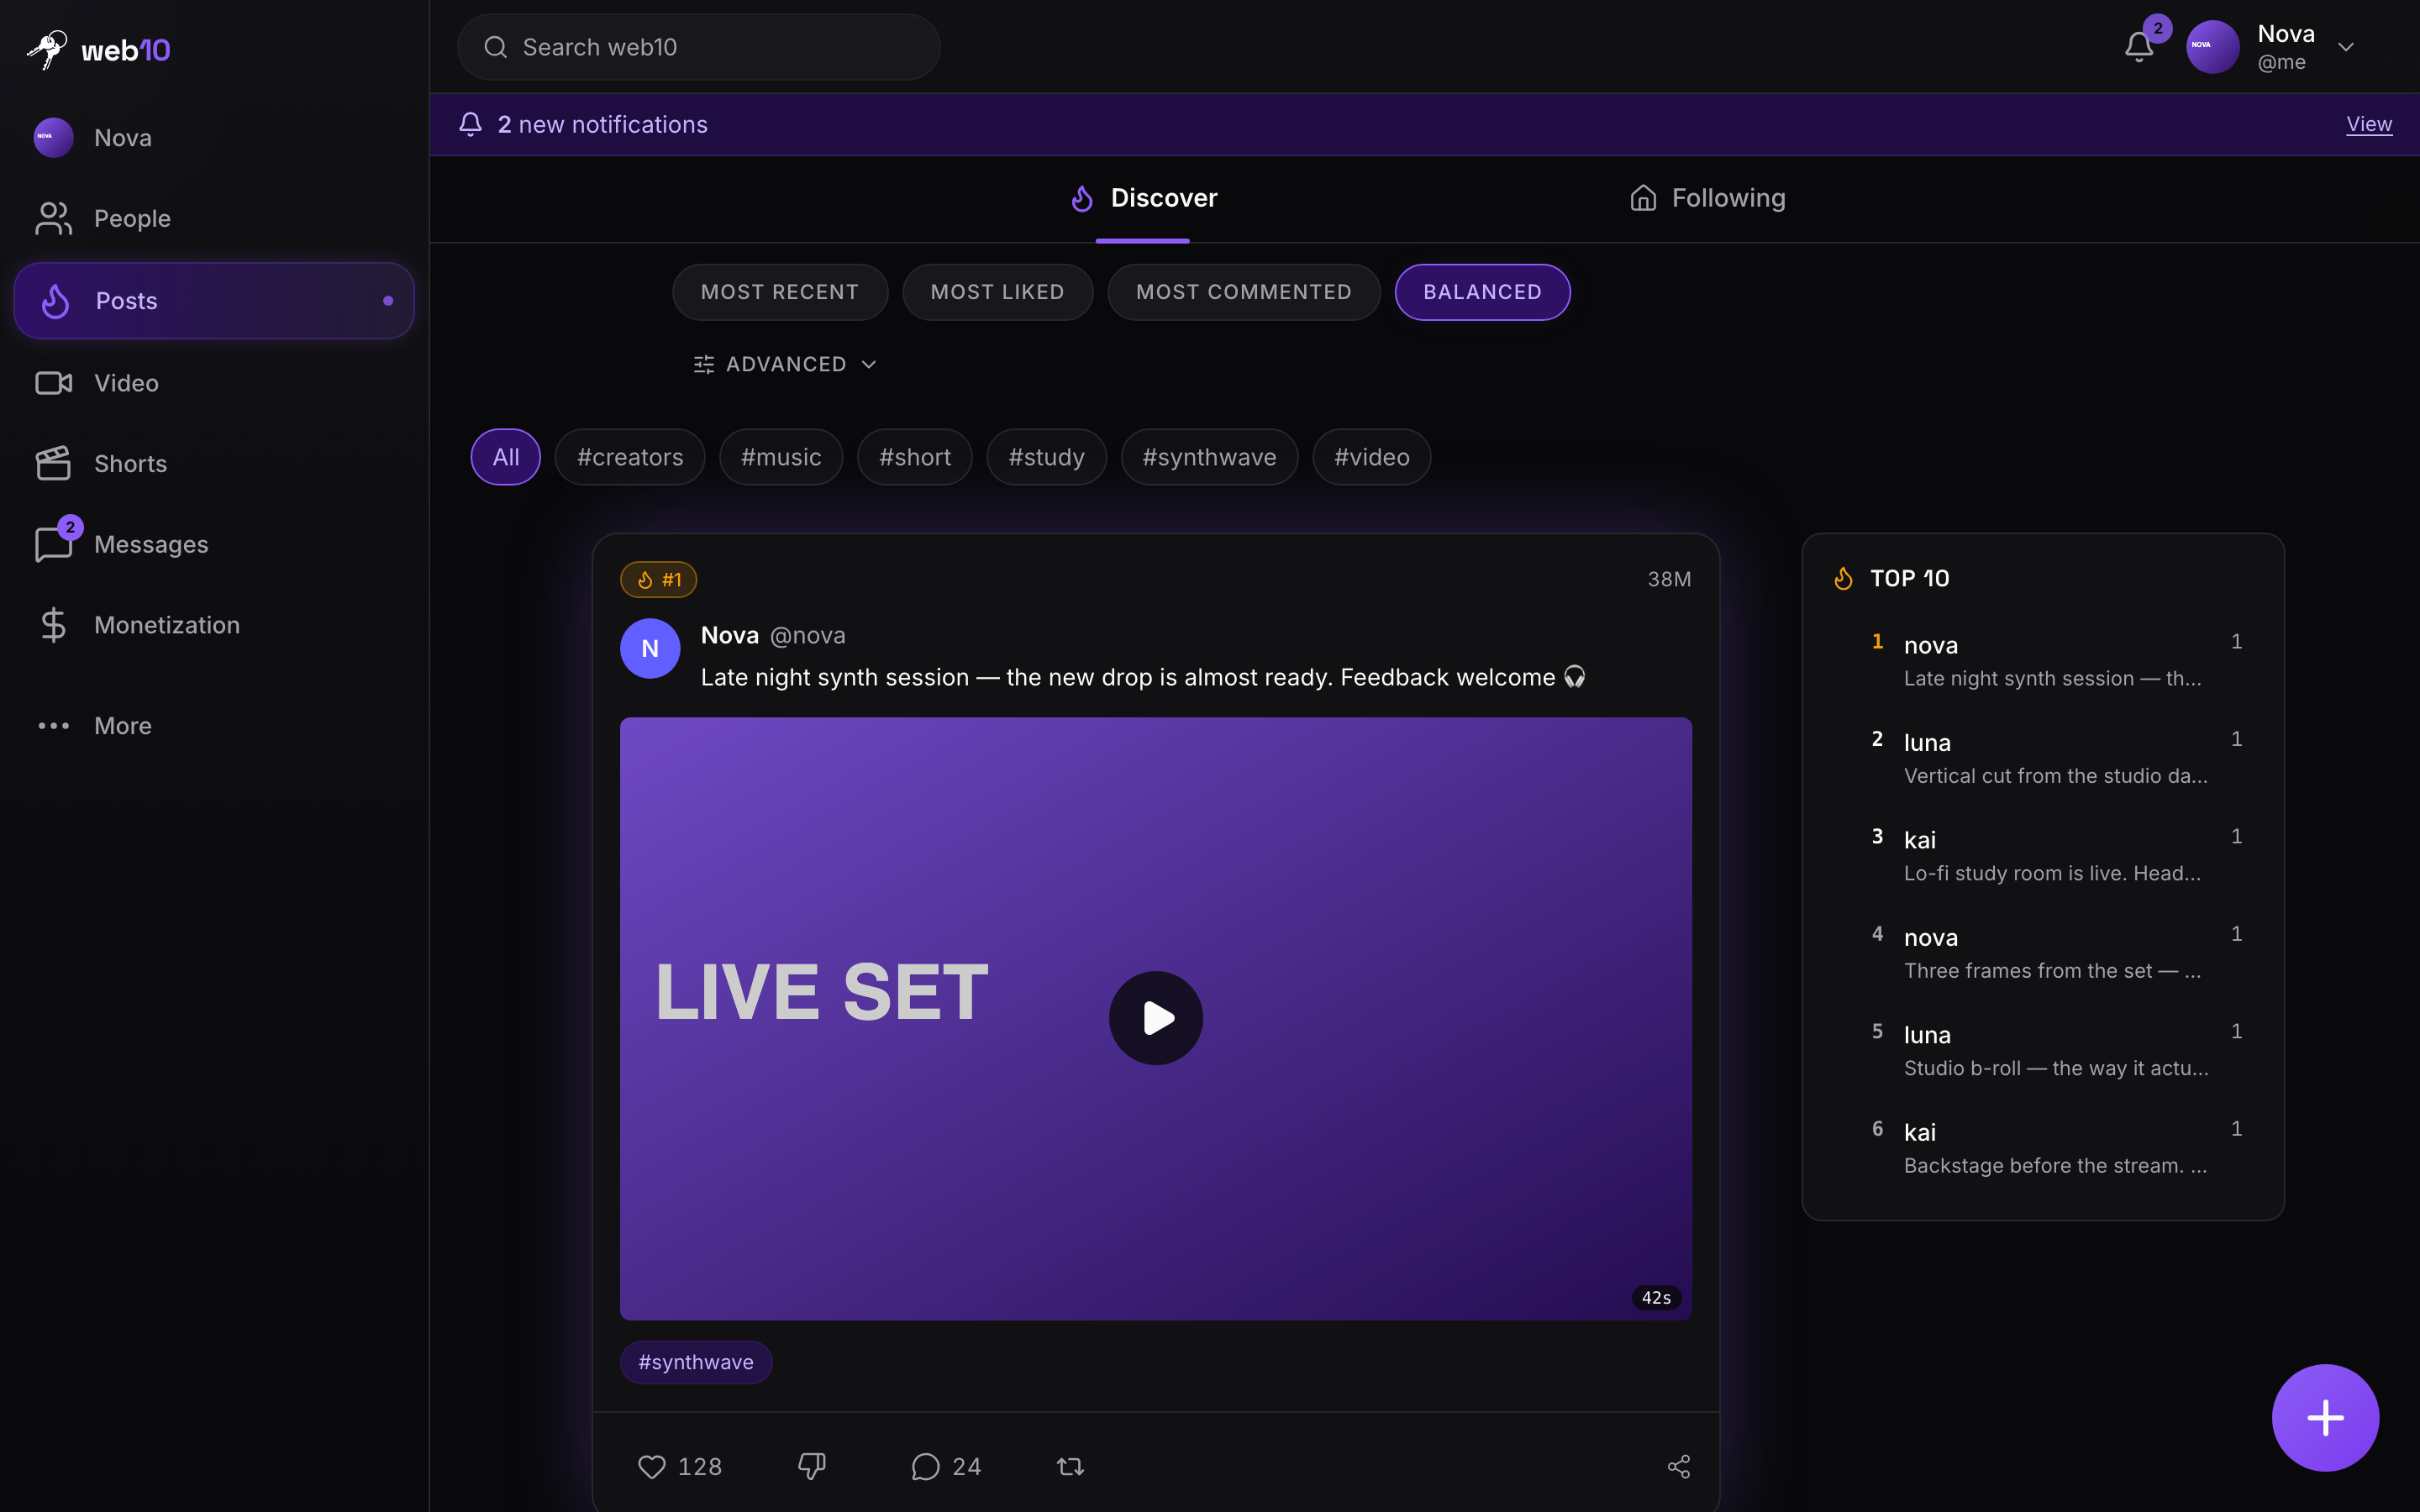
\includegraphics[width=\columnwidth]{figs/fig-feed.png}
  \caption{The web10 feed. The reader chooses the ranking (Most Recent / Most
  Liked / Most Commented / Balanced) and filters (tags); each is a different
  application query over the same columnar store. The main query uses
  reader-specific service boundaries; engagement and view metrics use
  follow-up calls.}
  \label{fig:feed}
\end{figure}

\begin{figure}[t]
  \centering
  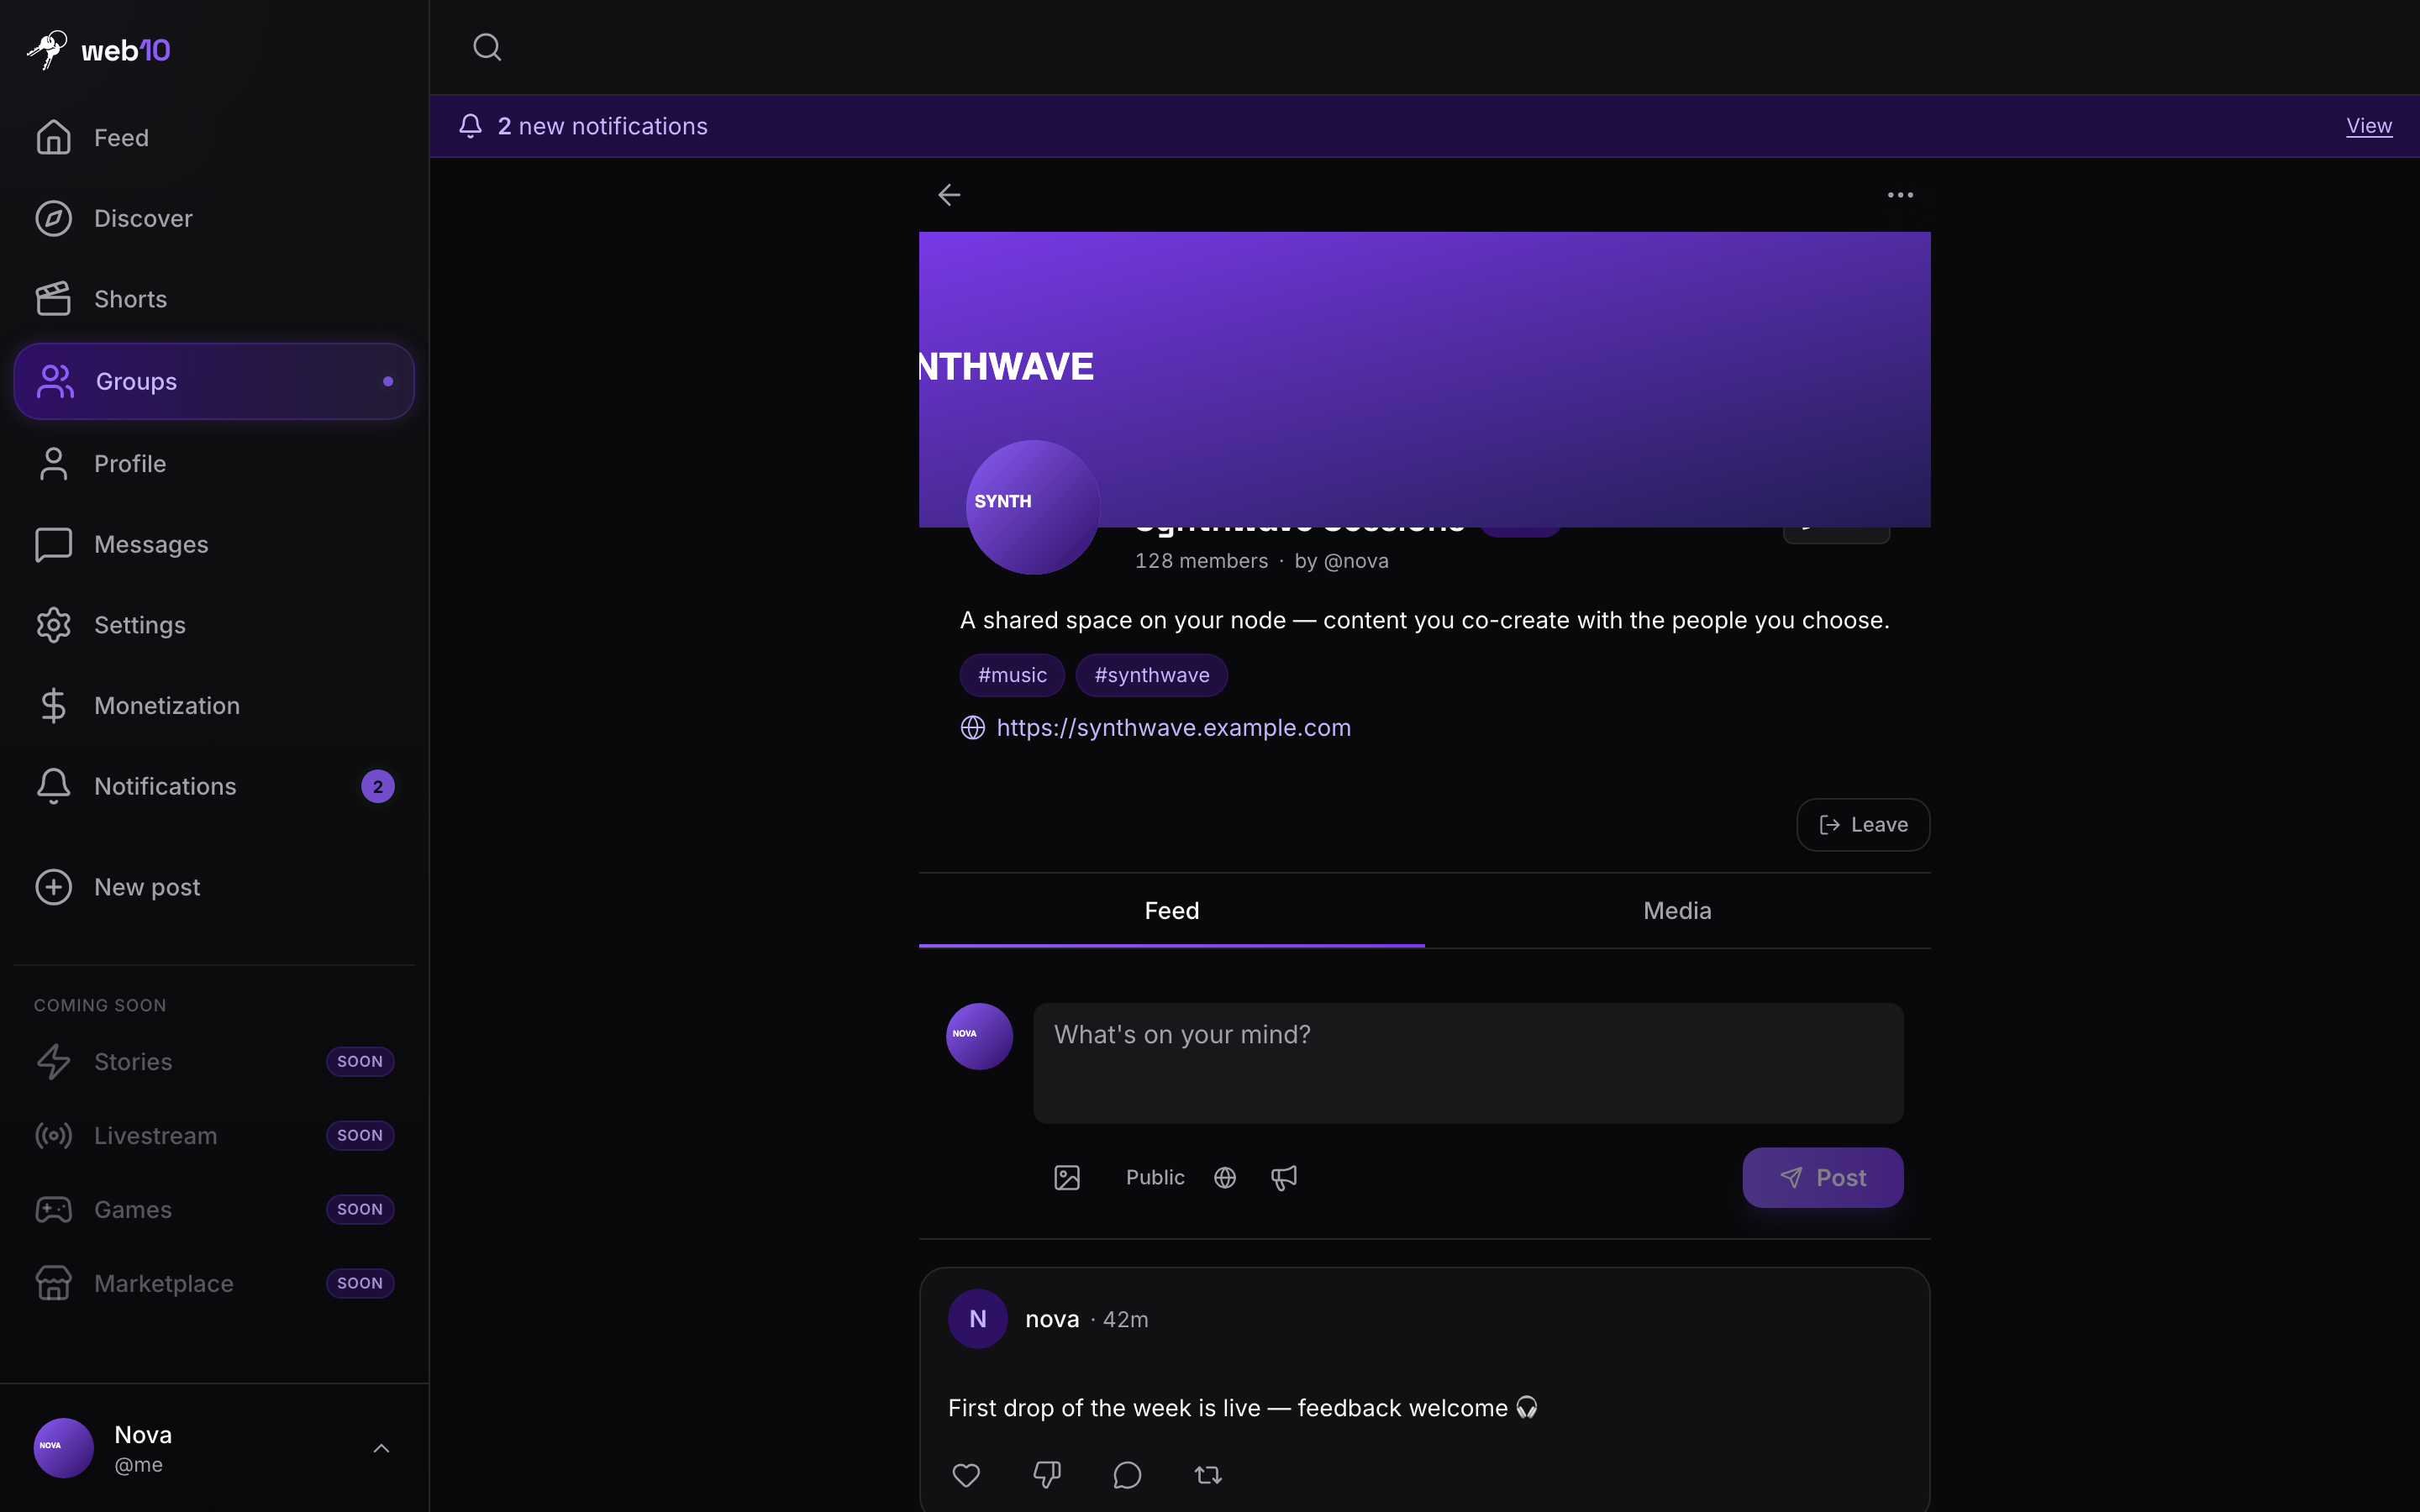
\includegraphics[width=\columnwidth]{figs/fig-groups.png}
  \caption{A group---``a shared space on your node.'' Membership, roles, and
  per-post visibility (Public / node / group) expose application choices over
  the generic groups and grants of \S\ref{sec:model}.}
  \label{fig:groups}
\end{figure}

\subsection{Multiple applications, one data plane}
\label{sec:platform:apps}

The social application is a \emph{producer} of reusable data, not the only
client of the node. Two small static applications consume its
\texttt{profile} documents: Snake associates completed runs with player
identities; Marketplace associates listings with seller identities. Each
writes its own service and reads the existing profile format
(Table~\ref{tab:interop-apps}). Neither modifies web10-social, and neither
adds a game, commerce, leaderboard, or seller-profile endpoint to the node.
The common dependency is the document convention and the access primitives---
not an application-specific API agreement.

\begin{table}[t]
  \caption{Data producers and consumers in the connected demonstration.
  Other social services are omitted.}
  \label{tab:interop-apps}
  \small
  \begin{tabular}{@{}lll@{}}
    \toprule
    Application & Writes & Reuses \\
    \midrule
    web10-social & \texttt{profile} & --- \\
    Snake & \texttt{snake\_scores} & \texttt{profile} \\
    Marketplace & \texttt{marketplace\_listings} & \texttt{profile} \\
    \bottomrule
  \end{tabular}
\end{table}

The following abbreviated leaderboard query illustrates the seam. Both
service names resolve to reader-filtered relations before the join; the full
application also selects each player's best score and supplies
profile-media preparation.

\begin{lstlisting}[style=sql]
WITH latest_profiles AS (
  SELECT author_key, body FROM profile
  QUALIFY row_number() OVER (
    PARTITION BY author_key
    ORDER BY updated_at DESC, created_at DESC,
             doc_id DESC) = 1
)
SELECT s.author_key,
       JSONExtractInt(s.body, 'score') AS score,
       p.body AS profile_body
FROM snake_scores s LEFT JOIN latest_profiles p
  ON s.author_key = p.author_key
ORDER BY score DESC LIMIT 50
\end{lstlisting}

Permission does not leak through the join. An application's permission to
read scores does not confer permission to read profiles, and an app-level
profile grant does not itself grant access to a private profile group. The
outer join can retain a score without a readable profile; the independent
group control in \S\ref{sec:interop-results} checks the corresponding
inner-join exclusion while the score records remain readable. Applications
therefore compose \emph{authorized relations}, not unrestricted copies of
another application's data.

Figure~\ref{fig:interop} shows the resulting player and seller identities.
The synthetic name was edited through the social UI, then read by both
applications; neither demo writes or recreates the profile. The connected
checks below verify the underlying records as well as their rendered names.

\begin{figure*}[t]
  \centering
  \begin{minipage}[t]{0.46\textwidth}
    \centering
    \textbf{Snake: earned score + social identity}\\[4pt]
    
\includegraphics[width=\linewidth]{../interoperability-demo/figures/snake-identity.png}
  \end{minipage}\hfill
  \begin{minipage}[t]{0.46\textwidth}
    \centering
    \textbf{Marketplace: listing + social identity}\\[4pt]
    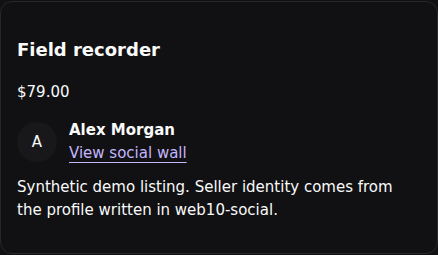
\includegraphics[width=\linewidth]{../interoperability-demo/figures/marketplace-identity.png}
  \end{minipage}
  \caption{One social-written profile, two application views. Snake joins an
  earned score to the player's profile; Marketplace joins a listing to the
  seller's same profile. These are direct browser element captures, with
  synthetic account and listing data. Full-page, consent, and denial captures
  are retained in the artifact.}
  \label{fig:interop}
\end{figure*}

\subsection{Durability and extensibility}

Application-named services let different clients interpret documents without
changing the shared document schema. A conversation can be a group with
message documents; a music library can define track services and listener
roles; a shop can define catalog services. Domain-specific transactions,
payment workflows, search indexes, schema evolution, and external
integrations can extend this common substrate.

The durable separation is between stored content/access relationships and a
particular frontend. Replacing a frontend can reuse those primitives when it
understands their semantics. The user-addressed network model of
\S\ref{sec:network} is the architectural answer to provider migration: the
user's principals and grants are globally addressable. Global addressing does
not itself migrate an account, its content, or its grants. The public
domain-subscription prototype exercises one continuity mechanism; complete
account/data migration and production cross-node integration remain outside
the demonstrated scope (\S\ref{sec:limits}).

%=============================================================================
\section{Lessons from Running It}
\label{sec:lessons}

The industry track asks what running a system taught you that designing it
did not. Four things, in roughly the order they bit.

\subsection{The node keeps resisting the killer app}

The platform's hardest dependency is its own killer app, and the killer app
is always going to ask for bespoke surface. A feed is faster to ship as an
endpoint than as a client query; a group's name, description, and banner
photo look like exactly the kind of thing a \texttt{group\_identity} table
would hold; a session oracle that knows about the followers group would make
the social app's re-authentication path trivial.

We built four such node surfaces, and we removed all four:

\begin{itemize}[leftmargin=*,nosep]
  \item a dedicated feed endpoint, replaced by an application-written query
  over the services it composes;
  \item a group-identity table with its own endpoint, replaced by documents
  in an app-named service read through the normal CRUD and grant path;
  \item a followers-group check inside the generic session oracle, moved to
  the one application that knows what a followers group is; and
  \item an ad path that hard-coded a collection name, replaced with a tag and
  group membership the applications themselves manage.
\end{itemize}

The test that caught each one is one sentence: \emph{would a notes app, a
music app, or a shop use this endpoint?} The moment the platform API grows a
table, function, or field that only makes sense for one application, another
application that defines identity differently---or has no followers
concept at all---cannot use the platform without the platform knowing its
specifics. The cost of holding the line is real and visible: the client does
more work. The feed is a composition the application writes, the
followers-group check lives in the social app, and publicness is a grant an
application adds rather than a flag a platform flips. The payoff is the
result in \S\ref{sec:platform:apps} and \S\ref{sec:interop-results}: a game
and a marketplace, with no relationship to the social application's code,
reading its profiles through the same boundary---and no node change when
either appeared.

\subsection{A self-healing schema raced its own readers}

On a fresh stack, the node self-heals its metadata schema with a deferred
\texttt{ALTER TABLE} at boot, adding columns to
\texttt{group\_contracts} that older databases lack. An early read that lands
before the \texttt{ALTER} commits fails with an unknown-identifier error, and
the failure is easiest to hit exactly where the stack is newest---a clean
database, a cold boot, the first request. The incident pins the fix: the
schema additions must land synchronously and be guaranteed before the first
read of that table, or the columns must exist at table creation, and the
regression that guards it boots a fresh database and immediately reads the
table. The general lesson is the one that survives the particular bug: a
self-heal that may lag is fine; a self-heal that may \emph{race} is not. Test
the fresh-boot path, not just the steady state.

\subsection{What the shared columnar table costs, day to day}

The data-plane choice of \S\ref{sec:data} trades physical isolation for
cross-author composition, and the running platform meets the price of that
trade every day: every read pays the version deduplication, because
\texttt{ReplacingMergeTree} only settles versions when it merges;
``deletion'' is an insert, so a tombstone is a row that must be ranked, not
discarded; merge pressure is background CPU that does not show up in request
latency until the host is busy; point queries are paid to an engine built
for scans; and every tenant in the node shares the same resources. These are
not defects of the design; they are the design's operating envelope, and the
reason the query boundary of \S\ref{sec:enforcement}---not a physical
partition---is where reader isolation lives.

\subsection{The first measurement pointed at the access layer, not the database}

The naive assumption is that a columnar engine will make reads cheap, so any
latency must live in the engine. The fan-out measurement of
\S\ref{sec:prelim} says the opposite at scale: with a reader following
1,000 creators, the per-group metadata resolver's median readable time was
7.64\,seconds while the document scan it fed was already done---the
authorization machinery, not the database, was the bottleneck. The batching
decision (three metadata queries plus in-memory resolution,
\S\ref{sec:prelim}) is the design consequence: the query endpoint should use
the batched resolver for large candidate sets. And the honest counterweight
is in the same table: at one candidate group, the per-group path is
\emph{faster}, because three fixed round trips dominate when there is one
group to check. The measurement that looks like an unqualified win is a
tradeoff with a knee; reporting both sides is the whole point of
\S\ref{sec:method}.

%=============================================================================
\section{Evaluation}
\label{sec:method}

The evaluation has five parts, and each part is organized as the question it
answers: does an unrelated application actually reuse another's data through
the access boundary (\S\ref{sec:interop-results})? Does a grant reach across
the node boundary, and can the owner revoke it locally
(\S\ref{sec:federation-results})? Does a public subscription outlive its
provider (\S\ref{sec:domain-results})? What does the access layer cost
(\S\ref{sec:prelim})? And is anyone actually using this
(\S\ref{sec:operating})? The first four use synthetic data on isolated test
stacks; the operating point is a read-only observation of the production
node. None is a capacity or scale result.

\subsection{Connected interoperability}
\label{sec:interop-results}

\emph{Question: do unrelated applications actually reuse each other's data,
through the access boundary, with consent and revocation exercised in a real
browser?}

\textbf{Browser reuse.} A fresh account logged into web10-social through its
authenticator popup and edited its profile name to Alex Morgan. The browser
approved Snake's app request, earned and saved ten points, and displayed the
joined profile. After app-contract revocation, a new query returned 403 and a
leaderboard refresh cleared the result and displayed an access error. After
sign-out, Marketplace requested its service permission through the popup,
published a listing, and displayed the same profile. Reloading the listing's
detail URL preserved that result. API assertions checked exact authors, row
counts, profile bodies and listing identity, so the username fallback alone
could not satisfy the test.

\textbf{Independent access controls.} A separate HTTP case used three
accounts and two social-written profiles. It checked exact two-author
score/profile and listing/profile joins. With no app permission for
\texttt{profile}, both queries were denied; granting it enabled the joins,
and revoking the app contract denied them again. A separately labeled
private-profile fixture isolated the group gate: membership enabled an exact
inner join; removal emptied it while the scores remained readable. The fixture
did not replace the social-written profiles in the reuse checks. HTTP
contracts were installed through the API; the browser sequence above
exercised the actual consent UI.

All three cases---desktop at 1440 pixels, mobile at 375 pixels, and HTTP
correctness---passed in the final fresh-stack run on 2 November 2026, with
zero retries or skips. Six flow captures and two identity-card captures per
viewport document the observed results.

\textbf{Setup and scope.} The run used a four-vCPU, 8-GB DigitalOcean sfo2
host, with ClickHouse 24.8.14.39, Playwright 1.63.0 and Chromium 153. The
artifact contains the exact experimental source, configuration, image
identities, results and all 16 original captures. The source includes local
modifications rather than an unmodified release; the complete snapshot is
retained in \domainartifactdir{research/interoperability-demo}{the
interoperability artifact}. The API, authenticator and social frontend used
development configurations; the marketing frontend used a production build.
Schema initialization preceded API startup. Project storage and the droplet
were removed after collection.

The hosted apps share one browser origin, although the HTTP case supplies a
separate app Origin. They demonstrate reuse across applications, not
separate-browser-origin isolation or an independently recruited developer
study. Clients know the profile format; automatic schema discovery is outside
this result. Initial-letter avatars are not media-delivery evidence. These
controls establish named grant/revocation behavior, not a stale-access or
capability-expiry bound.

\subsection{Cross-node identity and local revocation}
\label{sec:federation-results}

\emph{Question: does a grant really reach across the node boundary---and can
the owner revoke it locally?}

We ran a synthetic correctness scenario across two API processes, separate
ClickHouse and MinIO instances, independently generated HS256 signing
secrets, and real HTTPS home-issuer certification with an ephemeral test CA.
Bob creates a private group and document through B's API. Alice's
A-issued JWT initially fails both B's document read and query. This first
failure is the one that matters: giving a \emph{distinct B-side Alice} the
membership also fails to authorize A's Alice---two Alices, same name, and the
node tells them apart only through the qualified principal. Bob then grants
the exact foreign principal through the owner API. Both read paths return the
exact document; removing that membership denies both, and regrant restores
both.

All steps reuse the same JWT, and the certification traffic shows why the
model works the way \S\ref{sec:network} claims it does: A's TLS proxy records
exactly one successful certification across this entire lifecycle. B
rechecks access on every read while retaining the cached identity answer. A
foreign-provider JWT signed with B's key is rejected twice, with one failed
issuer call and a negatively cached second rejection. An independent
Origin-bearing query gate denies a local namesake's app grant, allows a
qualified foreign app-contract fixture, and denies again after its
revocation; direct group-authorized reads remain available.

The reported scenario completed without retries on an unmodified source
snapshot. It is a correctness experiment, not a deployment or load trial.
Docker-internal, globally classified addresses exercise the public-address
guard; the test CA and network do not establish public-internet
interoperability. Foreign app grant/revocation use labelled service-function
fixtures, not browser consent or completed foreign enrollment. Owner
grant/removal is not foreign self-join. Exact source, configuration, request
outcomes, image identities and cleanup records are retained in
\domainartifactdir{research/federation-demo}{the experiment artifact}, with
earlier attempts documented separately.

\subsection{Public domain subscriptions across provider loss}
\label{sec:domain-results}

\emph{Question: can a public subscription outlive the provider that hosts
it?}

A separate research client stores only a creator's normalized domain in a
private app document at the reader's independent home. It freshly resolves
the existing TXT pointer, checks the selected account's verified alias, and
reads public posts anonymously. It uses ordinary CRUD/groups and the existing
authenticated domain-verification endpoint---not a new node follow API.

On desktop (1440\,\texttimes\,1000) and mobile (375\,\texttimes\,812), the
creator logged in, copied/published the TXT, and verified the old account
through actual local UDP DNS. The reader clicked Follow once. Then the old
API/TLS services were stopped. With the original provider unavailable, the
creator retargeted DNS and verified a new account without the old provider's
approval. Reload and ordinary reader login displayed new public posts with
the identical stored follow ID/body and one total follow creation
(Figure~\ref{fig:domain-follow}). No old content was migrated. And the
asymmetry that should hold: explicit old private access returned 200 while
new-target private access remained 403---the public subscription follows the
domain, but private access is not inherited by the new target.

Additional controls delayed real responses at five identity-transition
boundaries and verified that logout or account changes prevented stale UI
updates. Missing or ambiguous DNS cleared displayed content without deleting
the saved subscription, and DNS/alias/public requests carried no credentials.
The experiment used an unmodified source snapshot. Exact source and
configuration, ten captures, request outcomes and cleanup records are
retained in \domainartifactdir{research/domain-portability-demo}{the
prototype artifact}.

This is a configured two-node client, not deployed social follows or private
principal continuity. API app/private grants, TTL-zero local DNS, a loopback
HTTP JSON bridge and browser acceptance of test-certificate errors are
explicit fixtures. Retained DNS control and available reader/new node/resolver
are assumptions; domain sale/theft/expiry and public DNS/TLS/availability are
not solved. The result demonstrates bounded public subscription continuity,
not absolute unbannability.

\begin{figure*}[t]
\centering
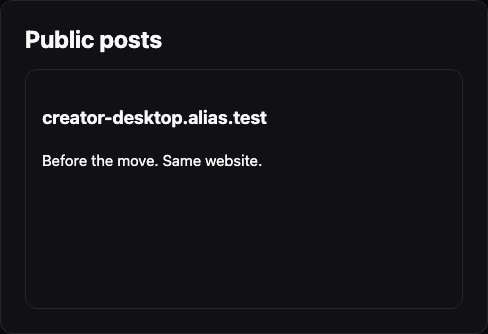
\includegraphics[width=.47\textwidth]{../domain-portability-demo/figures/before-card.png}\hfill
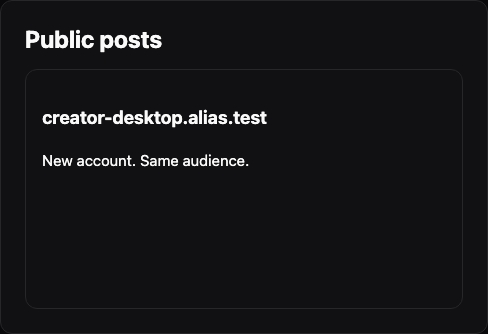
\includegraphics[width=.47\textwidth]{../domain-portability-demo/figures/after-card.png}
\caption{Same website, another public account. Exact panel crops from the
final desktop browser capture, before and after DNS retarget and old API/TLS
shutdown. The driver verifies the unchanged reader-owned follow ID and no
second Follow; full captures, authenticated hookup and 375px evidence remain
in the artifact.}
\label{fig:domain-follow}
\end{figure*}

\subsection{The metadata fan-out cost of the access layer}
\label{sec:prelim}

\emph{Question: what does the access layer cost, and where does the cost
live?}

The access layer resolves the reader's readable groups before the query
executes. We measured that cost to understand the design, not to report a
latency distribution: the question was whether per-group metadata resolution
scales with the number of candidate groups, and what a batched resolution
buys. Table~\ref{tab:fanout} reports one sequential trial on a DigitalOcean
sfo2 \texttt{s-4vcpu-8gb} host (four vCPUs, 8\,GB nominal RAM, Ubuntu 24.04,
Linux 6.8, Docker 29.1.3), co-locating a single Uvicorn process and
ClickHouse 24.3.18.7. The synthetic seed created 1,000 creators with one
small post each and a reader who joined all their groups; those groups also
granted public reads. Personal queries supplied $K=10$, $100$, or $1000$
candidate groups on this same dataset and host. A separate discover query
supplied one board group ($K=1$), containing ten additional posts. Queries
selected document IDs and bodies, ordered by creation time and ID, with a
limit of 20. They did not execute engagement joins, media preparation, or
browser page assembly. HTTP requests supplied no Origin header, so this
trial does not exercise the browser-origin app-contract gate.

\textbf{Variants.} The per-group resolver performs point metadata queries for
each candidate group. The batched resolver fetches memberships,
principal-class grants and role definitions across the candidate set in
three database queries, then resolves access in memory. This reduces round
trips, not the amount of permission metadata to process. We measured each
resolver with real document execution (B) and a fixed 20-row synthetic scan
result (C). C retains the policy/compilation path but is not an
output-equivalent query execution. A third variant (A) precompiles the
known-readable projection and times ClickHouse execution directly, outside
the HTTP handler.

\begin{table*}[t]
\centering
\small
\caption{Personal-query results from one sequential trial on the same
1,000-creator dataset, 20 samples per cell. B executes the document query; C
substitutes a fixed 20-row result. Times are milliseconds. Readable denotes
permission-resolution wall time; total denotes internal handler time, not
end-to-end HTTP latency.}
\label{tab:fanout}
\begin{tabular}{@{}rllrrrr@{}}
\toprule
$K$ & Resolver & Variant & Readable median & Readable p95 & Total median & Total p95 \\
\midrule
10 & Per-group & B & 75.03 & 93.30 & 129.36 & 171.18 \\
10 & Batched   & B & 23.47 & 31.17 & 81.28 & 98.91 \\
100 & Per-group & B & 764.39 & 843.21 & 831.35 & 915.18 \\
100 & Batched   & B & 41.78 & 51.65 & 99.42 & 139.47 \\
1000 & Per-group & B & 7535.71 & 8504.61 & 7644.66 & 8679.24 \\
1000 & Batched   & B & 213.98 & 284.03 & 363.31 & 435.03 \\
\midrule
10 & Per-group & C & 76.36 & 88.84 & 104.96 & 134.30 \\
10 & Batched   & C & 27.07 & 33.60 & 59.91 & 85.53 \\
100 & Per-group & C & 693.68 & 806.76 & 731.74 & 848.74 \\
100 & Batched   & C & 40.45 & 49.45 & 71.79 & 90.97 \\
1000 & Per-group & C & 8388.39 & 9102.21 & 8529.75 & 9204.19 \\
1000 & Batched   & C & 222.57 & 281.20 & 299.59 & 350.27 \\
\bottomrule
\end{tabular}
\end{table*}

\textbf{Finding.} The per-group resolver's cost grows linearly with the number
of candidate groups: increasing $K$ from 10 to 1,000 increased median
readable time by $100.44\times$. The batched resolver grows $9.12\times$ over
the same range---and at $K=1000$ reduces median readable time by $35.22\times$
and median handler time by $21.04\times$ relative to per-group. The
per-group path still completes requests, but its 7.64-second median at
$K=1000$ is a practical bottleneck for a reader who follows many creators;
the batched path's 363\,ms is not. This is the design decision the
measurement drives: the query endpoint should use the batched resolver for
large candidate sets.

The tradeoff is honest in both directions. Batching is not uniformly
cheaper: at the discover board's $K=1$, the per-group path is faster
(9.53\,ms readable versus 25.37\,ms batched), because three fixed round
trips dominate when there is one group to check. And batching does not make
the cost constant: the batched handler median still grew $4.47\times$ over
the 100-fold increase in $K$, as the metadata to process and the compiled
query to emit both grow with the candidate set. The result is a
characterization of the access layer's cost structure---metadata fan-out is
the dominant term at large $K$, and batching is the mitigation---not a claim
of constant latency or a performance benchmark.

The trial is a single sequential run (20 samples per cell, 400 measurements,
one host, localhost HTTP, no concurrency, no warm-up exclusion), and the
query is a simplified projection without engagement joins, media preparation,
or browser page assembly. It measures the access layer's cost structure on a
representative workload; it does not establish a latency distribution, a
capacity bound, or a causal authorization-overhead estimate. The direct-scan
baseline (A) excludes authentication, compilation, and serialization, so
$B - A$ is a pipeline-versus-scan comparison, not a matched causal
measurement. The trial used seed 42; exact source, configuration and
per-sample measurements are retained in
\domainartifactdir{research/experiments/costfn}{the measurement artifact}. An
earlier 100-creator trial on a different host and source snapshot showed the
same qualitative tradeoff and is not pooled with this table.

\subsection{A deployed operating point}
\label{sec:operating}

\emph{Question: is anyone actually using this?}

The platform is deployed and serving authenticated users. A read-only
observation of the production node on 28 October 2026 recorded 597 account
rows, 593 live documents across 30 distinct authors and 10 services, 49
group contracts, and 1,298 membership rows, on a host running the social,
authenticator, and API frontends. Nine authenticated browser navigations
(following feed, music, groups) returned HTTP 200 with a retained session and
zero uncaught page errors; the following feed rendered 20 posts in a median
5,396\,ms of full-page readiness. This is an operating point---evidence the
system runs and serves real users---not a capacity or scale result: the host
also runs a development stack, the observation is a snapshot without an
activity window, and the readiness figures include frontend startup and
network work, not server-query duration. The 5.4-second figure is the kind of
number the industry track exists to report: it is real, it is bad enough to
matter, and the full-feed measurement named in \S\ref{sec:limits} is the
dissection it asks for.

\subsection{Scope and open work}
\label{sec:limits}

The evaluation above is bounded by construction, and the open work is
specific.

\textbf{Federation beyond the correctness slice.} The isolated experiment in
\S\ref{sec:federation-results} exercises home-issuer certification and
owner-managed foreign grant/removal, not a complete federated product. The
domain prototype adds public subscription continuity, not production social
integration or private-principal portability. Independent production
signing-key provisioning, complete local-principal migration, foreign
self-join and app enrollment, multiworker/restart behavior, public deployment
and client-side feed merging remain open. Cached identity answers
intentionally last until JWT expiry; this does not establish immediate
issuer-side revocation or revoke already-issued media capabilities. JWKS
would be an optional verification optimization, not a prerequisite for the
live-call model.

\textbf{Workload and baseline.} The metadata fan-out measurement is a single
sequential trial on a simplified query. Full-feed latency (including
engagement joins, media preparation, and browser page assembly), concurrent
capacity, mixed allowed/denied access, and a matched shared-table policy
baseline (PostgreSQL with row-level security, same data and access
semantics) remain to be measured. A causal authorization-overhead estimate
requires an isolated ablation with equivalent preauthorized result sets, not
the pipeline-versus-scan comparison reported here.

\textbf{Correctness.} Security evidence consists of regression tests and the
named connected controls. Whole-system conformance, revocation-latency bounds
(racing grant changes with reads through metadata visibility, in-flight
requests, and issued capabilities), and the media capability boundary remain
open. Direct read-URL refresh enforces the verified caller's exact owner
namespace; that check alone does not establish stored-reference provenance or
revoke previously issued capabilities. Parser/engine semantic differences and
result-projection provenance require targeted testing.

%=============================================================================
\section{Related Work}
\label{sec:related}

The contribution is an integration of established ideas---user-addressed
storage, user-managed grants, and application-defined queries over
authorized relations. Table~\ref{tab:capabilities} organizes the comparison
along those dimensions; what follows is positioning, not a survey. We
discuss design differences from the cited systems rather than claiming that
no prior implementation combines these capabilities.

\textbf{Decentralized social data.}
ActivityPub~\cite{activitypub2018} (Mastodon) defines client/server and
federated server/server activity delivery; its authorization is
platform-defined---follow/block and collection-level visibility---not
per-principal grants over application-defined services.
ATProto~\cite{kleppmann2024} (Bluesky) separates repositories, relays, and
AppViews, supporting user agency and provider switching; its visibility model
is likewise collection-level, with AppViews providing application-defined
\emph{reads} but not user-managed \emph{grants}. These protocols organize
access around their social application models. web10 instead exposes
service-scoped roles to users and accepts application-defined SQL over the
resulting authorized relations---the seam that \S\ref{sec:platform:apps}
exercises with two applications that share nothing but the document
convention.

\textbf{Solid: the closest prior work.}
Solid~\cite{solid2016} separates applications from personal data stores
(Pods), with social application work~\cite{solid-apps2016} and a maintained
Community Solid Server~\cite{css2024}. WAC supports resource permissions and
group agents through \texttt{acl:agentGroup}~\cite{wac2022}, and ACP adds
agent, client, and issuer matching with allow/deny mode
sets~\cite{acp2022}. web10 does not claim Solid lacks group or client
authorization; it has both. The distinction is in the \emph{shape} of the
model. Solid's access control is \emph{resource-centric}---ACLs attached to
linked-data resources and containers, evaluated per resource. web10's is
\emph{service-centric}---a uniform role/grant vocabulary
(principal class $\times$ service $\times$ operation) in which a role is a
per-service permission map, the same shape across the app-trust and
person-trust layers, and the grant is a row naming a globally addressable
principal. Concretely: Solid answers ``who may read or write this
\emph{resource}?''; web10 answers ``what \emph{operations} may this
\emph{principal class} perform on this \emph{service}, in this
\emph{group}, under this \emph{app contract}?'' The latter is the IAM policy
shape (principal, service, operation, grant) exposed to the end user, not an
infrastructure operator. A second distinction is the query surface: Solid's
cross-Pod query cost depends on deployment, caching, and linked-data
traversal strategy; web10 composes application-defined SQL over a shared
columnar store with the access decision made on the input
(\S\ref{sec:enforcement}). A performance comparison would require a matched
workload and deployment; we do not claim one here.

\textbf{Cloud IAM and relationship-based authorization.}
AWS IAM (documentation)~\cite{awsiam} and the RBAC/ABAC
literature~\cite{ferraiolo1992, sandhu1996, abac2014} provide the policy
concepts web10 adapts at the user boundary: principals, roles,
service-scoped operations, revocable grants. The move is directional---a
familiar policy vocabulary exposed to \emph{users} about their own content
and groups, orchestrated by the API and query layer, rather than to
infrastructure operators about cloud resources. At industrial scale,
Zanzibar~\cite{zanzibar2019} is the closest prior art in
\emph{relationship-based} authorization: a uniform ACL data model and
configuration language across hundreds of services, with consistency as a
first-class problem (causal ordering of ACL updates, snapshot reads).
Zanzibar's model is \emph{infrastructure-side}---the operator defines the
relationship schema and the service enforces it, while applications can
expose sharing controls to their users. web10 explicitly exposes
service-scoped grants as user-managed data, names globally addressable
principals, and enforces access at the query layer over a shared columnar
store. Zanzibar's consistency guarantees motivate the explicit
revocation-visibility evaluation we leave as forward scope
(\S\ref{sec:limits}); we do not claim equivalent consistency here.
TAO~\cite{tao2013} provides the deployed precedent for \emph{read-time}
privacy checking at social-graph scale (a billion reads/sec, privacy check
per item, pull not push); web10's query boundary is the same idea---every
row access-checked on its way out---applied to service-namespaced documents
in a columnar store, with the check expressed as a reader-filtered CTE
rather than a per-item predicate.

\textbf{Multi-tenant isolation and row-level security.}
The database literature on tenant isolation---shared tables with an
organization identifier (Force.com~\cite{force2009}), schema-mapping
techniques~\cite{aulbach2008}, and the shared-versus-separate
spectrum~\cite{jacobs2007}---is the closest systems ancestor. web10's
key-space per user takes that spectrum to its limit: not one tenant per
organization, but one logical tenant per end user, in a shared columnar
store (\S\ref{sec:data}). Authorship uses \texttt{author\_key}; shared reads
use authorized group relations rather than a physical database boundary.
PostgreSQL row-security policies~\cite{postgres-rls} are the alternative
enforcement location: per-row policy evaluation inside the database engine.
web10 places enforcement above the engine---the reader-filtered CTE is
constructed in the application layer before the query reaches
ClickHouse~\cite{clickhouse2024}. Both placements can combine authorized
rows with application-defined joins and aggregation; a matched policy and
workload comparison (\S\ref{sec:method}) can distinguish the costs of these
placements. We report the design difference here and leave the cost
comparison as forward scope.

%=============================================================================
\section{Conclusion}
\label{sec:concl}

Email decentralized where your data goes; fifty years of practice show that
the model works at global scale, for one format, with the access layer left
behind. web10 is the generalization: a user-addressed network in which
applications define their own document services over a shared columnar store
in each sovereign node, in which a uniform, user-managed access model lets
any principal on any node hold a role in a user's groups, and in which the
query layer supplies the reader's service relations before joins and
aggregation execute. The cross-node boundary is the HTTP API and a verified
token---remote data is content, never control---and the client, not a
server-to-server relay, mediates the reads.

The evidence is connected, bounded, and named. A game and a marketplace
reuse the social application's profiles with no node change and no API
agreement, with browser consent and cross-author app/group controls
exercised end to end; a two-node experiment shows a foreign principal
granted, reading, revoked, and restored under a single cached
certification; a browser prototype keeps a public subscription alive after
its provider goes dark---while the private grants correctly stay behind.
And the metadata fan-out measurement identifies where the access layer's
cost actually lives at scale: at 1,000 candidate groups, batching reduced
median handler time from 7.64\,s to 363\,ms, while costing more at one
group. This is a design decision, not a scalability claim---and it is the
kind of concrete, measured tradeoff an operating system earns.

The forward scope is specific: federation beyond the isolated correctness
slice (\S\ref{sec:federation-results}), full-feed and concurrent workload
measurements, a matched shared-table policy baseline, and
revocation-latency bounds. The architectural contribution is the
integration itself: the email model, extended so that a user's permissions---
not just their data---leave the building with them.

%=============================================================================
\bibliographystyle{ACM-Reference-Format}
\bibliography{../references/web10-references}

\end{document}